\section{Creación de UAL Inventarium}\label{sec:4_web}
Este es la sección donde se juntan todos los conocimientos y herramientas que hemos ido exponiendo a lo largo de este documentos y los cohesionamos para crear UAL Inventarium.
\\UAL Inventarium o Inventarium es una herramienta web diseñada para la gestión del inventario del Departamento de Informática de la Universidad de Almería.
\\La página web está hecha en Angular 12. Angular es una plataforma de desarrollo compuesta por un framework y librerías. Angular nos brinda todas las herramientas necesarias para la creación de un sitio web.

\subsection{Estructura de un proyecto Angular}
Para poder desplegar un entorno donde trabajar en Angular primero hay que tenerlo instalado en Node Package Manager (NPM) con el siguiente comando:
\begin{verbatim}
    npm i -g @angular/cli
\end{verbatim}
Al hacer esto se desplegará el entorno de desarrollo para Angular. El directorio \textbf{node\_modules} es donde se almacena el Framework de Angular, el CLI y los distintos componentes que se vayan instalando con el NPM.
\begin{tcolorbox}
    [colback=green!5!white,colframe=green!75!black,fonttitle=\bfseries,title=¿Qué diferencias hay entre Angular CLI y Angular Framework?]
    Angular CLI es la Command Line Interface la cual permite poder crear proyectos Angular, añadir componentes, servicios o directivas desde una línea de comandos. Angular CLI se encarga de la gestión de las distintas posibilidades que puede ofrecer el framework de Angular.
\end{tcolorbox}
Los ficheros que se despliegan sobre el directorio raíz al crear un proyecto Angular \cite{angular-file-structure} son:
\begin{itemize}
    \item \textbf{.editorconfig}: Un archivo de configuración para editores de código.
    \item \textbf{README.MD}: Archivo de texto que procesa GitHub en sus repositorios. El contenido inicial del fichero en el momento de la creación del proyecto trata sobre documentación acerca del Framework.
    \item \textbf{angular.json}: Esta es la configuración predeterminada que aporta el CLI de Angular para poder construir la aplicación, generar el servicio y testear los diferentes componentes.
    \item \textbf{package.json}: Este fichero se encarga de manejar las dependencias de NPM, precisamente las que están habilitadas dentro del espacio de trabajo.
    \item \textbf{package-lock.json}: Aporta información del versionado de los distintos paquetes que están en node\_modules.
    \item \textbf{tsconfig.json}: Esta es la configuración básica de TypeScript para el proyecto.
    \item \textbf{proxy.conf.json}: Este es el fichero que va a ayudar a poder consumir la API. Reenvía las peticiones que llegan a la aplicación al puerto 3000 que es donde se encuentra ubicada.
\end{itemize}
En la misma carpeta raíz se tiene un directorio llamado \textit{src}, su descomposición es la siguiente:

\begin{itemize}
    \item \textbf{app}: Directorio que contiene todos los distintos componentes de los que está compuesta la aplicación.
    \item \textbf{assets}: Contiene imágenes y otros recursos para ser copiados en el momento que se construya la aplicación.
    \item \textbf{environments}: Gracias a este fichero puede configurarse una opción en particular de construcción de la aplicación.
    \item \textbf{favicon.ico}: El ícono que sale en la parte superior de la pestaña de la página web.
    \item \textbf{index.html}: La página principal que tiene cualquier web. El CLI se dedica a añadir automáticamente todo el JavaScript y el CSS cuando construye la aplicación. No es un fichero que se use.
    \item \textbf{main.ts}: Este fichero es el punto de entrada principal de la aplicación. Compila la aplicación y arranca el módulo raíz de la aplicación (AppModule) para que se ejecute en el navegador.
    \item \textbf{polyfills.ts}: Provee de adaptaciones para distintos navegadores.
    \item \textbf{styles.css}: Es un archivo de configuración global de estilos para todos los componentes de la aplicación.
    \item \textbf{test.ts}: El punto de entrada principal para los test que se realicen en la aplicación.
\end{itemize}

El contenido del directorio \textit{app} en el momento de la creación del proyecto es el siguiente:

\begin{itemize}
    \item \textbf{app.component.ts}: Define la lógica para la aplicación raíz.
    \item \textbf{app.component.html}: Define el diseño HTML asociaciado con el elemento raíz.
    \item \textbf{app.component.css}: Define el elemento de diseño para el elemento raíz.
    \item \textbf{app.component.spec.ts}: Define el conjunto de pruebas asociado con el elemento raíz.
    \item \textbf{app.module.ts}: Define el módulo raíz, este fichero le comunica a Angular cómo se tiene que realizar el ensamblaje de la aplicación. Inicialmente está declarado dentro de él el propio módulo raíz, pero a medida que se vayan añadiendo elementos a la aplicación se irán incluyendo más módulos.
\end{itemize}

Dentro de la carpeta \textit{src} hay tres directorios más:
\begin{itemize}
    \item \textit{components}.
    \item \textit{interfaces}.
    \item \textit{services}.
\end{itemize}
\subsubsection{Componente}
Los componentes son las estructuras principales de construcción que hay en Angular. Para poder generarlos se utiliza el siguiente comando:
\begin{verbatim}
    ng g c direccion_y_nombre_del_componente
\end{verbatim}
Cuando se ejecute se generará un nuevo directorio con el nombre del componente. Dentro de él se habrán creado cuatro ficheros diferentes:
\begin{itemize}
    \item \textbf{componente.html}: Aquí irá ubicado el diseño html que tendrá el componente.
    \item \textbf{componente.css}: Este documento de estilos se aplicará unicamente al componente.
    \item \textbf{componente.ts}: En el fichero TypeScript está la lógica del componente y cualquier tipo de procesado de datos que haya que realizar.
    \item \textbf{componente.spects.ts}: Este será el fichero de pruebas unitarias para el componente. Durante el desarrollo del proyecto no se ha utilizado ya que el testing del proyecto se ha hecho de otra forma.
\end{itemize}
\subsubsection{Servicio}
Los servicios sirven para aislar más el modelo de vista controlador que presentan los componentes. Estos serán los encargados de comunicarse con nuestra API.
\\Para generar un servicio se utiliza el siguiente comando:
\begin{verbatim}
    ng g s directorio_y_nombre_del_servicio
\end{verbatim}
Se generarán dos ficheros TypeScript, uno para el conjunto de pruebas y otro para el servicio.
\subsubsection{Interfaz}
La interfaz sirve para definir los elementos con los que se va a trabajar. Estos elementos corresponden a los que están en la base de datos.
\\Para poder generar una interfaz se escribe lo siguiente en la terminal dentro del proyecto:
\begin{verbatim}
    ng g i directorio_y_nombre_de_la_interfaz
\end{verbatim}
Un ejemplo de interfaz sería por ejemplo la de un objeto del tipo \textit{Configuración}:
\begin{verbatim}
    export interface Configuracion {
        idConfiguracion: number,
        ip: string,
        mac: string,
        boca: string,
        armario: string,
        usuario: string,
        contrasena: string,
        Objeto_idObjeto?: number
    }
\end{verbatim}
Estos elementos también ayudarán a procesar las respuestas que lleguen desde la API y para que puedan manipularse en los componentes de Angular sin problemas.
\subsection{Disposición y elementos que hay en Inventarium}
Se empezarán tratando los servicios y las interfaces y cómo se presenta su contenido en el caso de los primeros.

\subsubsection{Interfaces}
Se tiene una interfaz por cada elemento que se encuentra en la base de datos.

\subsubsection{Services}
Los servicios pueden ser los que hayan dado más tipos de problemas a lo largo del desarrollo. Son los encargados de generar las consultas HTTP de las que se han hablado en la sección anterior en el desarrollo de la API.
\\Se tienen tantos servicios como tablas en la base de datos quitando el de \textit{user} que sirve para iniciar sesión dentro de la aplicación.

\begin{figure}[h]
    \centering
    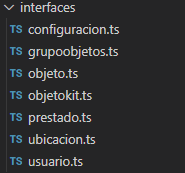
\includegraphics[keepaspectratio]{../contruccion_aplicacion/estructura_del_proyecto/interfaces.png}
    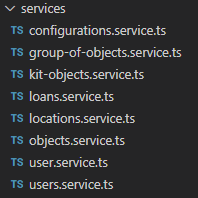
\includegraphics[keepaspectratio]{../contruccion_aplicacion/estructura_del_proyecto/servicios.png}
    \caption{Interfaces y servicios de UAL Inventarium}
\end{figure}

Para mostrar la estructura de uno de los servicios de la aplicación se verá como ejemplo el fichero \textit{group-of-objects.service.ts}. Al principio del documento están las importaciones de código y más adelante se declara lo siguiente:
\begin{verbatim}
    @Injectable({
        providedIn: 'root'
    })
\end{verbatim}
El \textit{@Injectable} junto al \textit{provideIn:`root'} sirve para que el servicio pueda utilizarse en todo el proyecto Angular.
\\Avanzando un poco más por el código puede observarse la declaración de la variable \textit{\_url} a la cual se le indica la dirección a la que tiene que mandar la solicitud.
\begin{verbatim}
    _url = "api/grupoobjetos"
\end{verbatim}
Como puede verse esa es la ruta a la que se accederá a la API. La dirección es así porque se ha habilitado un proxy que redirige las peticiones. De tal proxy se hablará más adelante.
\\En el constructor de la aplicación se inicializará la siguiente variable:
\begin{verbatim}
    constructor(private http: HttpClient) {}
\end{verbatim}
HttpClient es el servicio encargado de mandar las solicitudes HTTP a la API.
\\Ahora ya pueden empezarse a crear las funciones que se utilizarán a lo largo del desarrollo:
\begin{verbatim}
    getGroupOfObjects() {
        return this.http.get(this._url);
    }
\end{verbatim}
En este caso la petición que se manda es del tipo \textit{get} si se quiere crear un grupo de objetos sería con una petición \textit{post}:
\begin{verbatim}
    addGroupOfObject(objectGroup: FormData) {
        return this.http.post(this._url, objectGroup);
    }
\end{verbatim}
Donde como parámetro se pasa un campo del tipo formulario.
\\Para el resto de peticiones \textit{put} y \textit{delete} solamente se le añade un campo numérico que sea la id del objeto que se va a modificar \textit{/:id} y en el caso de put también se le pasa otro tipo de objeto formulario.
\\Con esto ya estaría definido el servicio listo para funcionar.
\subsection{Creación de componentes}
Ya sabemos cómo crear un componente pero no he explicado un poco de forma más detallada su funcionamiento.
\\Como ejemplo hablaremos de nuestro componente \textit{groups-of-objects} que es donde se visualizan todos los grupos de objetos.

\subsubsection{Preparar nuestro apartado TypeScript}
Declaramos las variables que necesitaremos, en este caso solo es una:
\begin{verbatim}
    group_of_objects: GrupoObjetos[] = [];
\end{verbatim}
Aprovechamos también para inicializar nuestro array de grupo de objetos. Como se puede ver al declarar la variable hemos llamado a su interfaz para que su utilización sea mucho más cómoda.
\\Para poder cargar los grupos de objetos que hay definidos en Inventarium tendremos que importar su servicio:
\begin{verbatim}
    constructor(private group_of_objects_service: GroupOfObjectsService)
\end{verbatim}
Y al querer que cuando accedamos a la página esta cargue los respectivos grupos de objetos, dentro del constructor tendremos que llamar al método para que lo haga:
\begin{verbatim}
    this.group_of_objects_service.getGroupOfObjects().subscribe(
    (data : any) => { 
        this.group_of_objects = res.data;
    },err => console.log('Error', err));
\end{verbatim}
El método \textit{getGroupOfObjects()} es el método que hemos definido anteriormente, el \textit{.subscribe} es para poder realizar la consulta. Dentro de él podremos decidir cómo manipular los elementos que nos devuelva la petición.
\\Este elemento es un objeto del \textit{json} pero Angular lo interpreta perfectamente. Objeto que puede tener uno de estos dos atributos, \textit{data} que es un array de grupo de objetos, significando que la consulta no ha tenido errores y \textit{err} que nos devuelve una cadena de carácteres en las que sale el tipo de error que ha ocurrido.
\\Con esto ya tendríamos nuestro objeto cargado, pero ahora tenemos que mostrarlo.
\subsubsection{Preparar nuestro archivo HTML}
Nuestro fichero HTML será el siguiente:
\begin{verbatim}
    <div class="row d-flex-inline justify-content-center">
    <!--Contenido-->
    <div *ngFor="let go of group_of_objects" style="width: fit-content;">
        <app-group-of-object>
            <img imagen class="card-img-top rounded-circle" 
            style="cursor:pointer" src="http://api/images/{{go.imagen}}.jpg">
            <h5 nombre [routerLink]="['/group-of-object', 
            go.idGrupoObjetos]" style="cursor:pointer"
            class="card-title text-dark text-center">
                {{go.nombre}}
            </h5>
            <span cantidad>{{go.cantidad}}</span>
            <span marca>{{go.marca}}</span>
            <span modelo>{{go.modelo}}</span>
            <span cantidadDisponible>{{go.cantidadDisponible}}</span>
            <span *ngIf="go.tipo==0" tipo>Inventario</span>
            <span *ngIf="go.tipo==1" tipo>Fungible</span>
            <span *ngIf="go.tipo==2" tipo>Kit</span>
        </app-group-of-object>
    </div>
</div>
\end{verbatim}
El componente es bastante sencillo. Primero definimos un contenedor donde iremos insertando tantos componentes nos haya devuelto la petición mandada anteriormente.
\\Ahora definimos otro contenedor donde iteraremos sobre nuestro array de groupo de objetos asignandolo a una variable auxiliar \textit{go}. Esto lo haremos utilizando \textit{*ngFor}.
\\Luego de iterar llamaremos a nuestro componente hijo que será el que iremos generando por cada grupo de objeto que cargue. Este componente lo veremos ahora después.
\\Dentro del componente hijo definiremos los componentes HTML que le queramos pasar. Para poder definir esto basta con añadirle un nombre que después referenciaremos en el otro componente.
\\Podemos ver al final del código que definimos un atributo dentro de nuestro componente HTML \textit{span} llamado \textit{*ngIf}. Este atributo es un condicional, en caso de que sea \textit{true} se cargará el componente. Si es \textit{false} no lo hará.
\\Ahora definiremos nuestro componente hijo que es al que estamos llamando:
\begin{verbatim}
    <div class="card border rounded p-3 m-2" 
    style="width: 22rem;background-color:#FDF7FF;">
    <div style="width: 100%; height: 230px;">
        <ng-content select="[imagen]"></ng-content>
    </div>
    <div style="width: 100%;" class="card-body list-group-item-dark border">
        <ng-content select="[nombre]"></ng-content>
    </div>
    <ul class="list-group list-group-flush">
        <li class="list-group-item bg-light">
            <b>Marca</b>
            <a>:<ng-content select="[marca]"></ng-content></a>
        </li>
        <li class="list-group-item bg-light">
            <b>Modelo</b>
            <a>:<ng-content select="[modelo]"></ng-content></a>
        </li>
        <li class="list-group-item bg-light">
            <b>Cantidad</b>
            <a>:<ng-content select="[cantidad]"></ng-content></a>
        </li>
        <li class="list-group-item bg-light">
            <b>Cantidad disponible</b>
            <a>:<ng-content select="[cantidadDisponible]"></ng-content></a>
        </li>
    </ul>
    <li class="list-group-item list-group-item-dark 
    font-weight-bold text-center">
        <ng-content select="[tipo]"></ng-content>
    </li>
    <ng-content select="[botones]"></ng-content>
</div>
\end{verbatim}
Este es el modelado que tiene nuestro objeto. El componente HTML llamado \textit{ng-content} será el encargado de tomar los objetos que le está pasando el componente padre. Estos los referencia con el atributo \textit{select} y le indica el nombre del tipo de componente que quiere coger.
\\Para poder ir revisando cómo quedan nuestros componentes utilizaremos una funcionalidad que nos incorpora Angular. Dentro de nuestro archivo \textit{package.json} NPM nos define una serie de scripts que podemos utilizar. Uno de ellos es el siguiente:
\begin{verbatim}
    "start": "ng serve"
\end{verbatim}
Para poder ejecutar este script ejecutaríamos el siguiente comando:
\begin{verbatim}
    npm run start
\end{verbatim}
Que sería lo mismo que utilizar:
\begin{verbatim}
    ng serve
\end{verbatim}
Esto nos despliega un servidor de la aplicación de Angular en el puerto 4200. Una de las ventajas que nos ofrece esto es una compilación continua del proyecto. Es decir, a medida que vayamos realizando la contruccion de la aplicación, la generación de componentes y la creación de rutas la web se irá actualizando en cada guardado y será de gran utilidad poder ir viendo estos cambios al momento.
\subsection{Definir el archivo de rutas}
Definir el archivo de rutas \cite{angular-routing} de la aplicación sirve para saber qué direcciones y que comportamientos tendrá esta en su uso.
\\Las rutas de la aplicación son las indicadas en la figura \ref{rutas_aplicacion}.

\begin{figure}[ht]
    \centering
    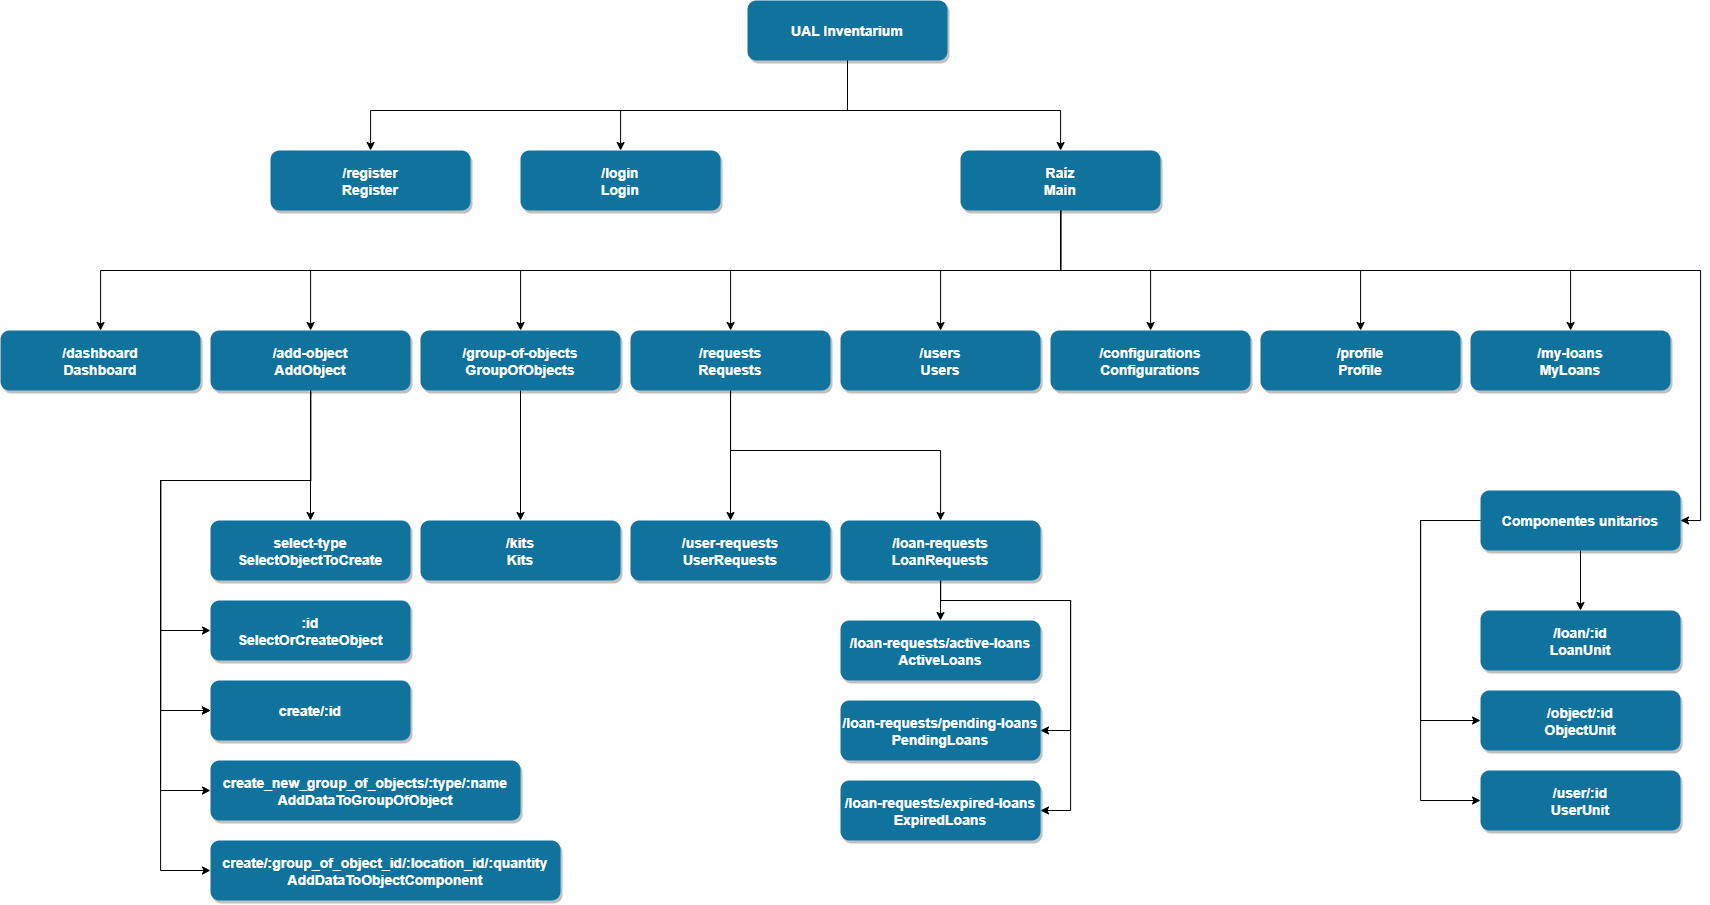
\includegraphics[width=\linewidth,keepaspectratio]{../contruccion_aplicacion/estructura_del_proyecto/app_routing.png}
    \caption{Rutas disponibles en la aplicación}\label{rutas_aplicacion}
\end{figure}

Las rutas de la aplicación tienen una correlación directa con el manejo de los componentes. Estas rutas se definen dentro del fichero \textit{app-routing.module.ts} que está dentro de \textit{app}.
\\Este archivo importa todos los componentes que vayan a utilizarse en las rutas. El comienzo del archivo consiste en definir una constante que se llamará routes y en la que irá toda la lógica de la aplicación:
\begin{verbatim}
    const routes: Routes = [
  {
    path: '', component: MainComponent,
    children: [
      { path: 'dashboard', component: DashboardComponent },
      {
        path: 'add-object', component: AddObjectComponent,
        children: [
          { path: 'select-type', component: SelectObjectToCreateComponent },
          .
          .
          .
\end{verbatim}
El archivo es bastante más extenso pero con este pequeño trozo pueden verse y explicarse los diferentes componentes que contiene.
\\Para definir una ruta de forma básica la estructura será la siguiente \textit{path: nombre\_de\_la\_ruta, component: nombre\_del\_componente} con esto al acceder a la ruta ya se mostraría dicho contenido.
\\Lo interesante que aporta Angular es la posibilidad de añadir hijos a estas rutas. Se hará llamando al atributo \textit{children: [array\_de\_rutas]}.
\\Esto es muy importante ya que el uso de hijos en las ruta hace que los componentes de rutas superiores no se descarguen. Se explicará mejor con el archivo \textit{MainComponent.html}:
\begin{verbatim}
<app-vertical-navbar></app-vertical-navbar>
<div class="page-content p-5" id="content">
    <!-- Toggle button -->
    <button id="sidebarCollapse" (click)="sidebarCollapse()" type="button"
    class="btn btn-light bg-white rounded-pill shadow-sm px-4 mb-4">
        <i class="fa fa-bars mr-2"></i>
        <small class="text-uppercase font-weight-bold">Toggle</small>
    </button>
    <router-outlet></router-outlet>
</div>
\end{verbatim}
Dentro del HTML se puede ver un componente llamativo: \textit{router-outlet}. Este está relacionado directamente con el routing que se tenga en la aplicación ya que es desde ahí donde se cargarán los hijos. La barra de navegación, por ejemplo, no desaparecería al acceder a \textit{/dashboard}.
\\Para realizar el importado de rutas dentro de Angular se llamará a \textit{\makeatletter@NgModule} al final del documento para que las exporte al componente principal.
\begin{verbatim}
    @NgModule({
        imports: [RouterModule.forRoot(routes)],
        exports: [RouterModule]
    })
\end{verbatim}
\subsection{Definir el proxy en nuestra aplicación}
La finalidad de un proxy inverso es reenviar las solicitudes que realiza la aplicación a la API, esta por políticas de CORS no puede reenviar una solicitud que entra al puerto 80 al puerto 3000 del mismo sitio. Tampoco se puede hacer que la API funcione sobre el puerto 80 ya que este puerto está siendo utilizado por la aplicación web. Por ello se tiene que hacer que este proceso se haga de forma interna en el servidor y para ello se utilizará un proxy inverso.
\\Un proxy inverso se encarga de reenviar las solicitudes que llegan a unas determinadas rutas del sitio web a otro puerto del entorno que no está alojado desde donde se envía. En este caso el proxy sería el encargado de que todas las solicitudes que entrasen por el puerto 80 de las direcciones definidas en la sección anterior sean redirigidas a la API que trabaja sobre el puerto 3000.
\\Este proxy inverso se definirá en el fichero \textit{proxy.conf.json} de la siguiente forma:
\begin{verbatim}
"/api/configuracion*": {
    "target": "http://localhost:3000",
    "changeOrigin": true
}
\end{verbatim}
Y para poder utilizarlo durante el desarrollo de la aplicación se modificará el comando que se utiliza para inicializar el entorno de pruebas por el siguiente:
\begin{verbatim}
    "start": "ng serve -o --proxy-config proxy.conf.json --host 0.0.0.0"
\end{verbatim}
\textit{/api/configuracion*} es para indicar que todas las solicitudes que llegen a la web con esa dirección se reenvien a \textit{"target": "http://localhost:3000"} y que se cambie el origen de la solicitud \textit{"changeOrigin": true}.
\begin{tcolorbox}
    [colback=green!5!white,colframe=green!75!black,fonttitle=\bfseries,title=¿Qué son las políticas de CORS?]
    CORS (Cross-Origin Resource Sharing) es un mecanismo o política de seguridad que permite controlar las peticiones HTTP asíncronas que se pueden realizar desde un navegador a un servidor con un dominio diferente de la página cargada originalmente. Este tipo de peticiones se llaman peticiones de origen cruzado (cross-origin). Estas peticiones no están permitidas por ley porque suelen ser utilizadas para la piratería informática.
\end{tcolorbox}
\subsection{Compilar el sitio Web}
Para compilar el sitio web es necesario ejecutar el siguiente comando dentro de la raíz del proyecto:
\begin{verbatim}
    ng build
\end{verbatim}
Esto generará un directorio \textit{dist} con otro directorio dentro con el nombre del proyecto. En este caso \textit{Inventarium}. Este contendrá todos los ficheros para poder añadirlo directamente a un servidor web.











